% Generated by pysimcount.pfoptimised -- do not edit; regenerate instead.
% CNOT total, cz, seed 10, merged, measured r; optimised = Nam Light marginal per step x r
% git_commit=e42ff29056ad9ea7fc7c9899fab334903e42e3e3 git_dirty=False
% derived: cnot-optimised.tex with Lie-Trotter S1 removed by pysimcount.figdrop (Lie-Trotter S1 alone spans 47% of the original y-axis); removed legends: Lie-Trotter S1, optimised; Lie-Trotter S1, unoptimised; source_sha256=771ca199a7b31ce13864c386afda3b4d256d5f53fb2504ed24b4b06d24d6f77e
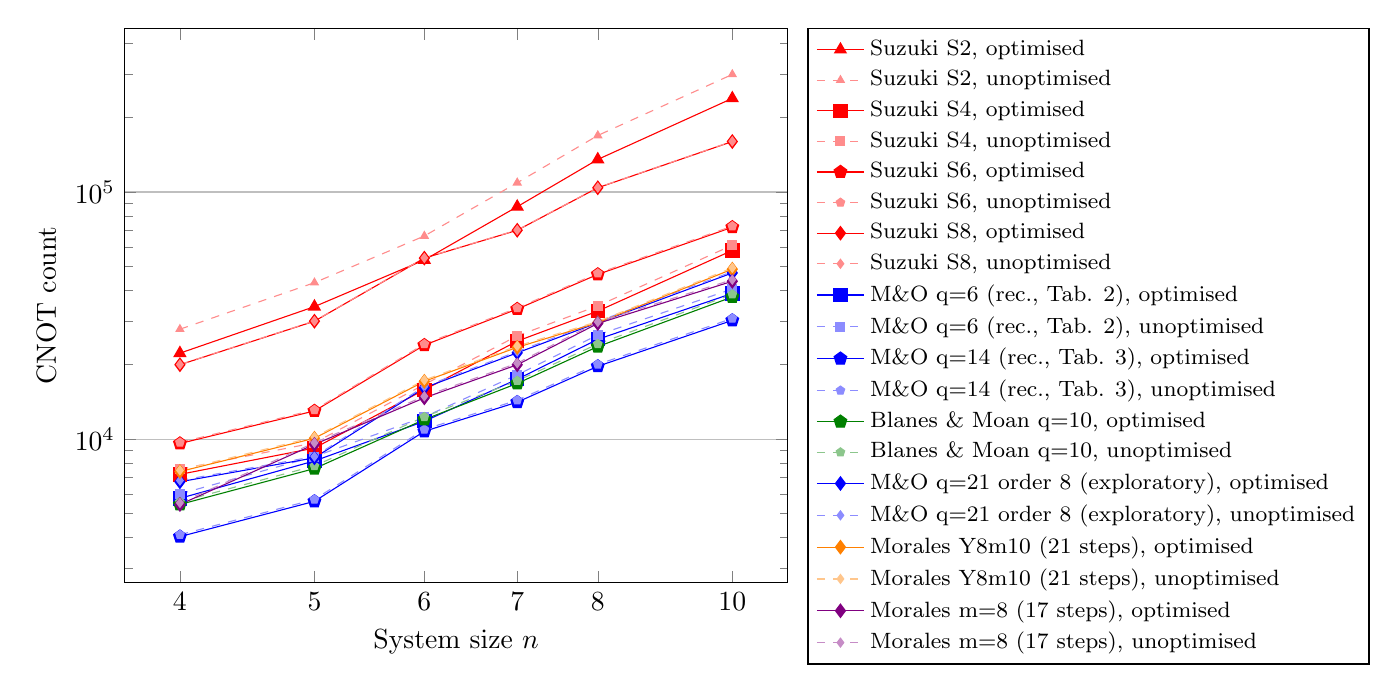
\begin{tikzpicture}
  \begin{loglogaxis}[
    width=10cm,
    xlabel={System size $n$},
    ylabel={CNOT count},
    xtick={4,5,6,7,8,10},
    xticklabels={4,5,6,7,8,10},
    ymajorgrids=true,
    legend pos=outer north east,
    legend cell align=left,
    legend style={font=\footnotesize},
  ]
    \addplot[red, mark=triangle*, mark size=2.4pt, mark options={solid, fill=red}] coordinates {
      (4,22272)
      (5,34360)
      (6,53088)
      (7,87192)
      (8,135424)
      (10,239200)
    };
    \addlegendentry{Suzuki S2, optimised}
    \addplot[red!45, dashed, mark=triangle*, mark size=1.6pt, mark options={solid, fill=red!45}] coordinates {
      (4,27840)
      (5,42950)
      (6,66360)
      (7,108990)
      (8,169280)
      (10,299000)
    };
    \addlegendentry{Suzuki S2, unoptimised}
    \addplot[red, mark=square*, mark size=2.4pt, mark options={solid, fill=red}] coordinates {
      (4,7200)
      (5,9200)
      (6,15840)
      (7,24920)
      (8,32960)
      (10,58000)
    };
    \addlegendentry{Suzuki S4, optimised}
    \addplot[red!45, dashed, mark=square*, mark size=1.6pt, mark options={solid, fill=red!45}] coordinates {
      (4,7560)
      (5,9660)
      (6,16632)
      (7,26166)
      (8,34608)
      (10,60900)
    };
    \addlegendentry{Suzuki S4, unoptimised}
    \addplot[red, mark=pentagon*, mark size=2.4pt, mark options={solid, fill=red}] coordinates {
      (4,9600)
      (5,13000)
      (6,24000)
      (7,33600)
      (8,46400)
      (10,72000)
    };
    \addlegendentry{Suzuki S6, optimised}
    \addplot[red!45, dashed, mark=pentagon*, mark size=1.6pt, mark options={solid, fill=red!45}] coordinates {
      (4,9696)
      (5,13130)
      (6,24240)
      (7,33936)
      (8,46864)
      (10,72720)
    };
    \addlegendentry{Suzuki S6, unoptimised}
    \addplot[red, mark=diamond*, mark size=2.4pt, mark options={solid, fill=red}] coordinates {
      (4,20000)
      (5,30000)
      (6,54000)
      (7,70000)
      (8,104000)
      (10,160000)
    };
    \addlegendentry{Suzuki S8, optimised}
    \addplot[red!45, dashed, mark=diamond*, mark size=1.6pt, mark options={solid, fill=red!45}] coordinates {
      (4,20040)
      (5,30060)
      (6,54108)
      (7,70140)
      (8,104208)
      (10,160320)
    };
    \addlegendentry{Suzuki S8, unoptimised}
    \addplot[blue, mark=square*, mark size=2.4pt, mark options={solid, fill=blue}] coordinates {
      (4,5760)
      (5,8160)
      (6,11808)
      (7,17472)
      (8,25344)
      (10,38880)
    };
    \addlegendentry{M\&O q=6 (rec., Tab. 2), optimised}
    \addplot[blue!45, dashed, mark=square*, mark size=1.6pt, mark options={solid, fill=blue!45}] coordinates {
      (4,6000)
      (5,8500)
      (6,12300)
      (7,18200)
      (8,26400)
      (10,40500)
    };
    \addlegendentry{M\&O q=6 (rec., Tab. 2), unoptimised}
    \addplot[blue, mark=pentagon*, mark size=2.4pt, mark options={solid, fill=blue}] coordinates {
      (4,4032)
      (5,5600)
      (6,10752)
      (7,14112)
      (8,19712)
      (10,30240)
    };
    \addlegendentry{M\&O q=14 (rec., Tab. 3), optimised}
    \addplot[blue!45, dashed, mark=pentagon*, mark size=1.6pt, mark options={solid, fill=blue!45}] coordinates {
      (4,4104)
      (5,5700)
      (6,10944)
      (7,14364)
      (8,20064)
      (10,30780)
    };
    \addlegendentry{M\&O q=14 (rec., Tab. 3), unoptimised}
    \addplot[green!50!black, mark=pentagon*, mark size=2.4pt, mark options={solid, fill=green!50!black}] coordinates {
      (4,5440)
      (5,7600)
      (6,12000)
      (7,16800)
      (8,23680)
      (10,37600)
    };
    \addlegendentry{Blanes \& Moan q=10, optimised}
    \addplot[green!50!black!45, dashed, mark=pentagon*, mark size=1.6pt, mark options={solid, fill=green!50!black!45}] coordinates {
      (4,5576)
      (5,7790)
      (6,12300)
      (7,17220)
      (8,24272)
      (10,38540)
    };
    \addlegendentry{Blanes \& Moan q=10, unoptimised}
    \addplot[blue, mark=diamond*, mark size=2.4pt, mark options={solid, fill=blue}] coordinates {
      (4,6720)
      (5,8400)
      (6,16128)
      (7,22344)
      (8,29568)
      (10,47040)
    };
    \addlegendentry{M\&O q=21 order 8 (exploratory), optimised}
    \addplot[blue!45, dashed, mark=diamond*, mark size=1.6pt, mark options={solid, fill=blue!45}] coordinates {
      (4,6800)
      (5,8500)
      (6,16320)
      (7,22610)
      (8,29920)
      (10,47600)
    };
    \addlegendentry{M\&O q=21 order 8 (exploratory), unoptimised}
    \addplot[orange, mark=diamond*, mark size=2.4pt, mark options={solid, fill=orange}] coordinates {
      (4,7392)
      (5,10080)
      (6,17136)
      (7,23520)
      (8,29568)
      (10,48720)
    };
    \addlegendentry{Morales Y8m10 (21 steps), optimised}
    \addplot[orange!45, dashed, mark=diamond*, mark size=1.6pt, mark options={solid, fill=orange!45}] coordinates {
      (4,7480)
      (5,10200)
      (6,17340)
      (7,23800)
      (8,29920)
      (10,49300)
    };
    \addlegendentry{Morales Y8m10 (21 steps), unoptimised}
    \addplot[violet, mark=diamond*, mark size=2.4pt, mark options={solid, fill=violet}] coordinates {
      (4,5440)
      (5,9520)
      (6,14688)
      (7,19992)
      (8,29376)
      (10,43520)
    };
    \addlegendentry{Morales m=8 (17 steps), optimised}
    \addplot[violet!45, dashed, mark=diamond*, mark size=1.6pt, mark options={solid, fill=violet!45}] coordinates {
      (4,5520)
      (5,9660)
      (6,14904)
      (7,20286)
      (8,29808)
      (10,44160)
    };
    \addlegendentry{Morales m=8 (17 steps), unoptimised}
  \end{loglogaxis}
\end{tikzpicture}
